\chapter{Results}
\label{sec:results}


\section{Presentation of Collected Data}
\subsection{Overview of Interviews}
We conducted semi-structured interviews with 16 native Swedish speakers (10 M/6F, age 23-78), each lasting 1-3 minutes. Each participant was interviewed for two different scenarios, resulting in 30 different recordings. All interviews were audio-recorded in a quiet room and elicited two target emotions – anger and happiness – via open-ended prompts (e.g. “Is there anything in society that makes you upset? What? How does that make you feel?”; “Can you remember one time you felt really proud of yourself?”). The participants rated their perceived emotions on a 1-6 scale immediately after each scenario. The rated emotions covered the basic 5 emotions mentioned in this report: anger, joy, sadness, fear, and surprise. 

Table~\ref{tab:interview_table} presents the participants ID, gender, age, and self-assessed scores for their perceived emotions for respective interview scenario.
\begin{table}[H]
    \centering
    \begin{tabular}{|lrl|
    >{\columncolor[HTML]{FBE2D5}}l 
    >{\columncolor[HTML]{FBE2D5}}l 
    >{\columncolor[HTML]{FBE2D5}}l 
    >{\columncolor[HTML]{FBE2D5}}l 
    >{\columncolor[HTML]{FBE2D5}}l |
    >{\columncolor[HTML]{DAF2D0}}l 
    >{\columncolor[HTML]{DAF2D0}}l 
    >{\columncolor[HTML]{DAF2D0}}l 
    >{\columncolor[HTML]{DAF2D0}}l 
    >{\columncolor[HTML]{DAF2D0}}l |}
    \hline
    \multicolumn{3}{|c|}{Participant}                                                                                                 & \multicolumn{5}{c|}{\cellcolor[HTML]{F7C7AC}Negative}                                                                                                                                                     & \multicolumn{5}{c|}{\cellcolor[HTML]{B5E6A2}Positive}                                                                                                                                                                                                  \\ \hline
    \multicolumn{1}{|l|}{\cellcolor[HTML]{D9D9D9}ID} & \multicolumn{1}{l|}{\cellcolor[HTML]{D9D9D9}M/F} & \cellcolor[HTML]{D9D9D9}Age & \multicolumn{1}{l|}{\cellcolor[HTML]{FBE2D5}A} & \multicolumn{1}{l|}{\cellcolor[HTML]{FBE2D5}J} & \multicolumn{1}{l|}{\cellcolor[HTML]{FBE2D5}Sad} & \multicolumn{1}{l|}{\cellcolor[HTML]{FBE2D5}F} & Sur & \multicolumn{1}{c|}{\cellcolor[HTML]{DAF2D0}A} & \multicolumn{1}{c|}{\cellcolor[HTML]{DAF2D0}J} & \multicolumn{1}{c|}{\cellcolor[HTML]{DAF2D0}Sad} & \multicolumn{1}{c|}{\cellcolor[HTML]{DAF2D0}F} & \multicolumn{1}{c|}{\cellcolor[HTML]{DAF2D0}Sur} \\ \hline
    \multicolumn{1}{|l|}{1}                          & \multicolumn{1}{r|}{M}                           & 23                          & \multicolumn{1}{l|}{\cellcolor[HTML]{FBE2D5}5} & \multicolumn{1}{l|}{\cellcolor[HTML]{FBE2D5}1} & \multicolumn{1}{l|}{\cellcolor[HTML]{FBE2D5}3}   & \multicolumn{1}{l|}{\cellcolor[HTML]{FBE2D5}1} & 1   & \multicolumn{1}{l|}{\cellcolor[HTML]{DAF2D0}1} & \multicolumn{1}{l|}{\cellcolor[HTML]{DAF2D0}6} & \multicolumn{1}{l|}{\cellcolor[HTML]{DAF2D0}1}   & \multicolumn{1}{l|}{\cellcolor[HTML]{DAF2D0}1} & 4                                                \\ \hline
    \multicolumn{1}{|l|}{2}                          & \multicolumn{1}{r|}{M}                           & 26                          & \multicolumn{1}{l|}{\cellcolor[HTML]{FBE2D5}6} & \multicolumn{1}{l|}{\cellcolor[HTML]{FBE2D5}1} & \multicolumn{1}{l|}{\cellcolor[HTML]{FBE2D5}3}   & \multicolumn{1}{l|}{\cellcolor[HTML]{FBE2D5}4} & 1   & \multicolumn{1}{l|}{\cellcolor[HTML]{DAF2D0}1} & \multicolumn{1}{l|}{\cellcolor[HTML]{DAF2D0}6} & \multicolumn{1}{l|}{\cellcolor[HTML]{DAF2D0}1}   & \multicolumn{1}{l|}{\cellcolor[HTML]{DAF2D0}2} & 1                                                \\ \hline
    \multicolumn{1}{|l|}{3}                          & \multicolumn{1}{r|}{F}                           & 27                          & \multicolumn{1}{l|}{\cellcolor[HTML]{FBE2D5}4} & \multicolumn{1}{l|}{\cellcolor[HTML]{FBE2D5}1} & \multicolumn{1}{l|}{\cellcolor[HTML]{FBE2D5}6}   & \multicolumn{1}{l|}{\cellcolor[HTML]{FBE2D5}1} & 2   & \multicolumn{1}{l|}{\cellcolor[HTML]{DAF2D0}1} & \multicolumn{1}{l|}{\cellcolor[HTML]{DAF2D0}6} & \multicolumn{1}{l|}{\cellcolor[HTML]{DAF2D0}1}   & \multicolumn{1}{l|}{\cellcolor[HTML]{DAF2D0}1} & 3                                                \\ \hline
    \multicolumn{1}{|l|}{4}                          & \multicolumn{1}{r|}{M}                           & 29                          & \multicolumn{1}{l|}{\cellcolor[HTML]{FBE2D5}2} & \multicolumn{1}{l|}{\cellcolor[HTML]{FBE2D5}1} & \multicolumn{1}{l|}{\cellcolor[HTML]{FBE2D5}3}   & \multicolumn{1}{l|}{\cellcolor[HTML]{FBE2D5}2} & 1   & \multicolumn{1}{l|}{\cellcolor[HTML]{DAF2D0}1} & \multicolumn{1}{l|}{\cellcolor[HTML]{DAF2D0}4} & \multicolumn{1}{l|}{\cellcolor[HTML]{DAF2D0}2}   & \multicolumn{1}{l|}{\cellcolor[HTML]{DAF2D0}2} & 2                                                \\ \hline
    \multicolumn{1}{|l|}{5}                          & \multicolumn{1}{r|}{F}                           & 28                          & \multicolumn{1}{l|}{\cellcolor[HTML]{FBE2D5}4} & \multicolumn{1}{l|}{\cellcolor[HTML]{FBE2D5}1} & \multicolumn{1}{l|}{\cellcolor[HTML]{FBE2D5}4}   & \multicolumn{1}{l|}{\cellcolor[HTML]{FBE2D5}1} & 2   & \multicolumn{1}{l|}{\cellcolor[HTML]{DAF2D0}1} & \multicolumn{1}{l|}{\cellcolor[HTML]{DAF2D0}5} & \multicolumn{1}{l|}{\cellcolor[HTML]{DAF2D0}1}   & \multicolumn{1}{l|}{\cellcolor[HTML]{DAF2D0}1} & 5                                                \\ \hline
    \multicolumn{1}{|l|}{6}                          & \multicolumn{1}{r|}{M}                           & 25                          & \multicolumn{1}{l|}{\cellcolor[HTML]{FBE2D5}2} & \multicolumn{1}{l|}{\cellcolor[HTML]{FBE2D5}2} & \multicolumn{1}{l|}{\cellcolor[HTML]{FBE2D5}1}   & \multicolumn{1}{l|}{\cellcolor[HTML]{FBE2D5}1} & 1   & \multicolumn{1}{l|}{\cellcolor[HTML]{DAF2D0}1} & \multicolumn{1}{l|}{\cellcolor[HTML]{DAF2D0}3} & \multicolumn{1}{l|}{\cellcolor[HTML]{DAF2D0}1}   & \multicolumn{1}{l|}{\cellcolor[HTML]{DAF2D0}1} & 1                                                \\ \hline
    \multicolumn{1}{|l|}{8}                          & \multicolumn{1}{r|}{M}                           & 27                          & \multicolumn{1}{l|}{\cellcolor[HTML]{FBE2D5}3} & \multicolumn{1}{l|}{\cellcolor[HTML]{FBE2D5}1} & \multicolumn{1}{l|}{\cellcolor[HTML]{FBE2D5}2}   & \multicolumn{1}{l|}{\cellcolor[HTML]{FBE2D5}1} & 2   & \multicolumn{1}{l|}{\cellcolor[HTML]{DAF2D0}1} & \multicolumn{1}{l|}{\cellcolor[HTML]{DAF2D0}5} & \multicolumn{1}{l|}{\cellcolor[HTML]{DAF2D0}1}   & \multicolumn{1}{l|}{\cellcolor[HTML]{DAF2D0}1} & 1                                                \\ \hline
    \multicolumn{1}{|l|}{9}                          & \multicolumn{1}{r|}{F}                           & 26                          & \multicolumn{1}{l|}{\cellcolor[HTML]{FBE2D5}3} & \multicolumn{1}{l|}{\cellcolor[HTML]{FBE2D5}1} & \multicolumn{1}{l|}{\cellcolor[HTML]{FBE2D5}3}   & \multicolumn{1}{l|}{\cellcolor[HTML]{FBE2D5}1} & 1   & \multicolumn{1}{l|}{\cellcolor[HTML]{DAF2D0}1} & \multicolumn{1}{l|}{\cellcolor[HTML]{DAF2D0}5} & \multicolumn{1}{l|}{\cellcolor[HTML]{DAF2D0}1}   & \multicolumn{1}{l|}{\cellcolor[HTML]{DAF2D0}1} & 1                                                \\ \hline
    \multicolumn{1}{|l|}{10}                         & \multicolumn{1}{r|}{F}                           & 78                          & \multicolumn{1}{l|}{\cellcolor[HTML]{FBE2D5}5} & \multicolumn{1}{l|}{\cellcolor[HTML]{FBE2D5}1} & \multicolumn{1}{l|}{\cellcolor[HTML]{FBE2D5}3}   & \multicolumn{1}{l|}{\cellcolor[HTML]{FBE2D5}2} & 4   & \multicolumn{1}{l|}{\cellcolor[HTML]{DAF2D0}1} & \multicolumn{1}{l|}{\cellcolor[HTML]{DAF2D0}6} & \multicolumn{1}{l|}{\cellcolor[HTML]{DAF2D0}4}   & \multicolumn{1}{l|}{\cellcolor[HTML]{DAF2D0}1} & 1                                                \\ \hline
    \multicolumn{1}{|l|}{11}                         & \multicolumn{1}{r|}{F}                           & 27                          & \multicolumn{1}{l|}{\cellcolor[HTML]{FBE2D5}3} & \multicolumn{1}{l|}{\cellcolor[HTML]{FBE2D5}3} & \multicolumn{1}{l|}{\cellcolor[HTML]{FBE2D5}2}   & \multicolumn{1}{l|}{\cellcolor[HTML]{FBE2D5}1} & 1   & \multicolumn{1}{l|}{\cellcolor[HTML]{DAF2D0}1} & \multicolumn{1}{l|}{\cellcolor[HTML]{DAF2D0}6} & \multicolumn{1}{l|}{\cellcolor[HTML]{DAF2D0}1}   & \multicolumn{1}{l|}{\cellcolor[HTML]{DAF2D0}1} & 1                                                \\ \hline
    \multicolumn{1}{|l|}{12}                         & \multicolumn{1}{r|}{M}                           & 58                          & \multicolumn{1}{l|}{\cellcolor[HTML]{FBE2D5}1} & \multicolumn{1}{l|}{\cellcolor[HTML]{FBE2D5}3} & \multicolumn{1}{l|}{\cellcolor[HTML]{FBE2D5}1}   & \multicolumn{1}{l|}{\cellcolor[HTML]{FBE2D5}2} & 1   & \multicolumn{1}{l|}{\cellcolor[HTML]{DAF2D0}1} & \multicolumn{1}{l|}{\cellcolor[HTML]{DAF2D0}6} & \multicolumn{1}{l|}{\cellcolor[HTML]{DAF2D0}1}   & \multicolumn{1}{l|}{\cellcolor[HTML]{DAF2D0}1} & 3                                                \\ \hline
    \multicolumn{1}{|l|}{13}                         & \multicolumn{1}{r|}{F}                           & 54                          & \multicolumn{1}{l|}{\cellcolor[HTML]{FBE2D5}4} & \multicolumn{1}{l|}{\cellcolor[HTML]{FBE2D5}1} & \multicolumn{1}{l|}{\cellcolor[HTML]{FBE2D5}4}   & \multicolumn{1}{l|}{\cellcolor[HTML]{FBE2D5}3} & 1   & \multicolumn{1}{l|}{\cellcolor[HTML]{DAF2D0}1} & \multicolumn{1}{l|}{\cellcolor[HTML]{DAF2D0}6} & \multicolumn{1}{l|}{\cellcolor[HTML]{DAF2D0}1}   & \multicolumn{1}{l|}{\cellcolor[HTML]{DAF2D0}1} & 1                                                \\ \hline
    \multicolumn{1}{|l|}{14}                         & \multicolumn{1}{r|}{M}                           & 20                          & \multicolumn{1}{l|}{\cellcolor[HTML]{FBE2D5}1} & \multicolumn{1}{l|}{\cellcolor[HTML]{FBE2D5}3} & \multicolumn{1}{l|}{\cellcolor[HTML]{FBE2D5}1}   & \multicolumn{1}{l|}{\cellcolor[HTML]{FBE2D5}2} & 2   & \multicolumn{1}{l|}{\cellcolor[HTML]{DAF2D0}1} & \multicolumn{1}{l|}{\cellcolor[HTML]{DAF2D0}4} & \multicolumn{1}{l|}{\cellcolor[HTML]{DAF2D0}1}   & \multicolumn{1}{l|}{\cellcolor[HTML]{DAF2D0}1} & 3                                                \\ \hline
    \multicolumn{1}{|l|}{15}                         & \multicolumn{1}{r|}{M}                           & 30                          & \multicolumn{1}{l|}{\cellcolor[HTML]{FBE2D5}3} & \multicolumn{1}{l|}{\cellcolor[HTML]{FBE2D5}2} & \multicolumn{1}{l|}{\cellcolor[HTML]{FBE2D5}2}   & \multicolumn{1}{l|}{\cellcolor[HTML]{FBE2D5}3} & 1   & \multicolumn{1}{l|}{\cellcolor[HTML]{DAF2D0}2} & \multicolumn{1}{l|}{\cellcolor[HTML]{DAF2D0}5} & \multicolumn{1}{l|}{\cellcolor[HTML]{DAF2D0}1}   & \multicolumn{1}{l|}{\cellcolor[HTML]{DAF2D0}1} & 1                                                \\ \hline
    \multicolumn{1}{|l|}{16}                         & \multicolumn{1}{r|}{M}                           & 25                          & \multicolumn{1}{l|}{\cellcolor[HTML]{FBE2D5}4} & \multicolumn{1}{l|}{\cellcolor[HTML]{FBE2D5}1} & \multicolumn{1}{l|}{\cellcolor[HTML]{FBE2D5}2}   & \multicolumn{1}{l|}{\cellcolor[HTML]{FBE2D5}1} & 1   & \multicolumn{1}{l|}{\cellcolor[HTML]{DAF2D0}1} & \multicolumn{1}{l|}{\cellcolor[HTML]{DAF2D0}6} & \multicolumn{1}{l|}{\cellcolor[HTML]{DAF2D0}1}   & \multicolumn{1}{l|}{\cellcolor[HTML]{DAF2D0}1} & 1                                                \\ \hline
    \end{tabular}
    \caption{Participant table. A: Anger, J: Joy, Sad: Sadness, F: Fear, Sur: Surprise.}
    \label{tab:interview_table}
\end{table}

\subsection{Data Collection for RQ1: Vocal Features \& Speech}

\subsubsection{Pipeline Overview}
text ? kanske inte ha med vet ej 

\subsubsection{Structure of JSON Data Files}
\begin{center}
\begin{minipage}{0.7\textwidth} 
\begin{lstlisting}[language=json, caption={Example of stored JSON structure for vocal features vs. Hume}]
    {
    "entry_id": "id_005_neg",
    "vocal_features": {
        "mean_pitch_st": -4.12,
        "mean_pitch_hz": 118.24,
        "mean_intensity_db": 58.15,
        "mean_hnr_db": -0.5,
        "jitter_local": 0.0261,
        "shimmer_local": 0.1096,
        "formants_hz": {
            "F1": 1118.56,
            "F2": 2623.03,
            "F3": 3611.26
        }
    },
    "praat_scores": {
        "anger": 0.208,
        "joy": 0.205,
        "fear": 0.199,
        "sadness": 0.19,
        "surprise": 0.198
    },
    "praat_label": "anger",
    "hume_probs": {
        "anger": 0.21,
        "fear": 0.16,
        "joy": 0.15,
        "sadness": 0.34,
        "surprise": 0.14
    },
    "hume_label": "sadness"
}
\end{lstlisting}
\end{minipage}
\end{center} 
\subsubsection{Segment-Level Data}
text

\subsection{Data Collection for RQ2 and RQ3: Text, Speech and Self-Assessment}


The data collection for RQ2 and RQ3 is based on the same audio recordings as for RQ1. 
Each recording was transcribed and analyzed with NLP Cloud (text-based), to extract emotion probabilities from the transcription. The same audio was analyzed using Hume AI for speech-based emotion detection, resulting in paired emotion probability scores alongside self-reported emotion ratings. All scores were normalized for comparison.

The data was structured in JSON format as shown in Figure~\ref{tab:json_rq2_rq3}, each audio object consists of five emotion labels from each data type (Hume, NLP, Self). 

\begin{center}
    \begin{minipage}{0.7\textwidth} 
    \begin{lstlisting}[language=json, caption={Example of stored JSON structure for Hume, NLP, Self-labeling.}]
        {
            "id_013_neg": {
                "audio_file": "audio_use/negative/13-neg.m4a",
                "nlp_emotions": {
                    "anger": 0.44,
                    "joy": 0.0,
                    "sadness": 0.31,
                    "fear": 0.21,
                    "surprise": 0.05
                },
                "hume_emotions": {
                    "anger": 0.32,
                    "fear": 0.13,
                    "joy": 0.22,
                    "sadness": 0.19,
                    "surprise": 0.13
                },
                "self_assessed": {
                    "anger": 0.31,
                    "joy": 0.08,
                    "sadness": 0.31,
                    "fear": 0.23,
                    "surprise": 0.08
                }
            }
    }
    \end{lstlisting}
    \label{tab:json_rq2_rq3}
\end{minipage}
\end{center} 

Table~\ref{tab:summery_rq2_rq3} summarize the average emotion scores and standard deviations for both speech-based (Hume AI) and text-based (NLP Cloud) 
models across all clips in the dataset. 

\begin{table}[H]
    \begin{tabular}{c|l|l|l|l|l|l}
    \textbf{Emotion}  & \multicolumn{1}{c|}{\textbf{Self Mean}} & \multicolumn{1}{c|}{\textbf{Hume Mean}} & \multicolumn{1}{c|}{\textbf{NLP Mean}} & \multicolumn{1}{c|}{\textbf{Self Std}} & \multicolumn{1}{c|}{\textbf{Hume Std}} & \multicolumn{1}{c}{\textbf{NLP Std}} \\ \hline
    \textbf{Anger}    & 0,21                                               & 0,26                                    & 0,2                                    & 0,124                                           & 0,072                                  & 0,223                                \\
    \textbf{Joy}      & 0,312                                              & 0,302                                   & 0,396                                  & 0,2                                             & 0,117                                  & 0,351                                \\
    \textbf{Sadness}  & 0,19                                               & 0,167                                   & 0,181                                  & 0,105                                           & 0,065                                  & 0,138                                \\
    \textbf{Fear}     & 0,136                                              & 0,15                                    & 0,093                                  & 0,061                                           & 0,045                                  & 0,092                                \\
    \textbf{Surprise} & 0,149                                              & 0,118                                   & 0,129                                  & 0,082                                           & 0,022                                  & 0,089                               
    \end{tabular}
    \caption{Mean and standard deviation for Hume, NLP, Self-labeling for full dataset.}
    \label{tab:summery_rq2_rq3}
\end{table}

The interviews are directed either positively or negatively. 
The data from these interviews are structured as the Table 

\begin{table}[H]
    \begin{tabular}{lllll}
    \multicolumn{5}{c}{\cellcolor[HTML]{BFBFBF}Negative}                                                                                                                                                \\ \hline
    \multicolumn{1}{|l|}{\textbf{Emotion}}  & \multicolumn{1}{c|}{\textbf{Hume M}} & \multicolumn{1}{c|}{\textbf{NLP M}} & \multicolumn{1}{c|}{\textbf{Hume Sd}} & \multicolumn{1}{c|}{\textbf{NLP Sd}} \\ \hline
    \multicolumn{1}{|l|}{\textbf{Anger}}    & 0,29                                 & 0,363                               & 0,072                                 & 0,183                                \\ \cline{1-1}
    \multicolumn{1}{|l|}{\textbf{Joy}}      & 0,276                                & 0,121                               & 0,098                                 & 0,205                                \\ \cline{1-1}
    \multicolumn{1}{|l|}{\textbf{Sadness}}  & 0,171                                & 0,282                               & 0,066                                 & 0,104                                \\ \cline{1-1}
    \multicolumn{1}{|l|}{\textbf{Fear}}     & 0,152                                & 0,141                               & 0,038                                 & 0,087                                \\ \cline{1-1}
    \multicolumn{1}{|l|}{\textbf{Surprise}} & 0,112                                & 0,092                               & 0,021                                 & 0,064                                \\ \cline{1-1}
    \end{tabular}
    \caption{Mean and standard deviation for Hume and NLP for negative interviews.}
    \label{tab:summery_hume_nlp_neg}
\end{table}


\begin{table}[H]
    \begin{tabular}{lllll}
    \multicolumn{5}{c}{\cellcolor[HTML]{BFBFBF}Positive}                                                                                                                                           \\
    \multicolumn{1}{l|}{\textbf{Emotion}}  & \multicolumn{1}{c}{\textbf{Hume M}} & \multicolumn{1}{c}{\textbf{NLP M}} & \multicolumn{1}{c}{\textbf{Hume Sd}} & \multicolumn{1}{c}{\textbf{NLP Sd}} \\ \hline
    \multicolumn{1}{l|}{\textbf{Anger}}    & 0,228                               & 0,015                              & 0,06                                 & 0,057                               \\
    \multicolumn{1}{l|}{\textbf{Joy}}      & 0,334                               & 0,708                              & 0,132                                & 0,168                               \\
    \multicolumn{1}{l|}{\textbf{Sadness}}  & 0,164                               & 0,067                              & 0,065                                & 0,062                               \\
    \multicolumn{1}{l|}{\textbf{Fear}}     & 0,148                               & 0,04                               & 0,053                                & 0,068                               \\
    \multicolumn{1}{l|}{\textbf{Surprise}} & 0,126                               & 0,171                              & 0,022                                & 0,097                              
    \end{tabular}
    \caption{Mean and standard deviation for Hume and NLP for positive interviews.}
    \label{tab:summery_hume_nlp_pos}
\end{table}

\section{Data Analysis for RQ1: Vocal Features \& Speech Emotion Recognition}
text 
\subsection{Correlation Between Vocal Features and AI Emotion Scores (Hume AI)}

\begin{figure}[H]
    \centering
    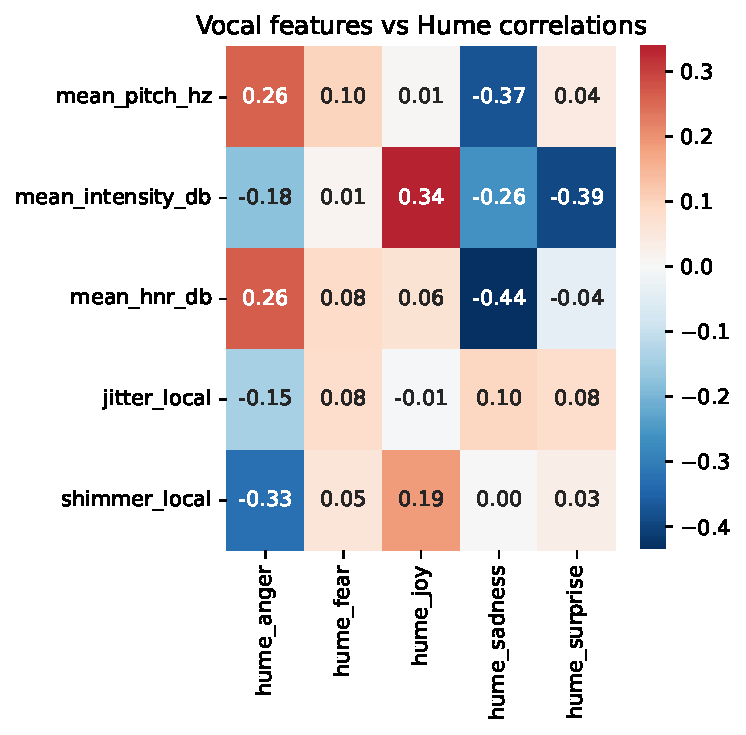
\includegraphics[width=0.6\textwidth]{png/results/rq1/vocal_features_vs_hume_correlations.pdf}
    \caption{Heatmap of correlation between vocal markers and Hume labels.}
    \label{fig:heatmap-voc-hume}
\end{figure}

Figure~\ref{fig:heatmap-voc-hume} demonstrates a heatmap of the Pearson correlation coefficients between selected vocal features and Hume AI emotion labels across all clips in the dataset. The results show generally weak correlations, with most values in the range of -0.4 and 0.3. 

\medskip
Key findings: 
\begin{itemize}
    \item Mean pitch (Hz) shows a moderate correlation with both anger (r = 0.26) and surprise (r = 0.04). This partially aligns with expectations from the previous research \autocite{Ekberg2023}, that showed elevated pitch was associated with high-arousal emotions such as anger and joy. 
    \item Mean Intensity (dB) has a positive correlation with joy (r = 0.34) and a negative correlation with sadness (r = -0.26) and surprise (r = -0.39). These results align with the referred research indicating that vocal intensity tends to increase with positive arousal states \autocite{Ekberg2023}. 
    \item Mean HNR has a slightly positive correlation with anger (r = 0.26), but shows weak correlations across all other emotions.
    \item Jitter and shimmer showed weak correlations, which may reflect that these features are subtle in spontaneous speech contexts compared to controlled or acted settings.  
\end{itemize}
Overall, the correlations with Hume suggest minor tendencies that reflect known vocal-emotion relationships, especially regarding pitch and intensity. The low degree of these correlations indicates that selected acoustic features alone did not strongly predict AI-detected emotions. 

\subsection{Correlation with Praat-Based Emotion Scores}

\begin{figure}[H]
    \centering
    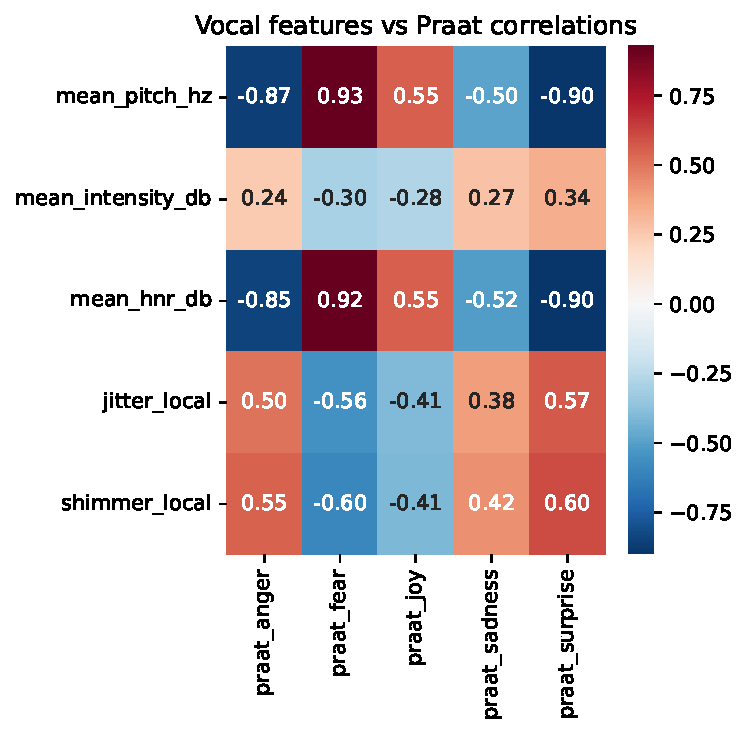
\includegraphics[width=0.6\textwidth]{png/results/rq1/vocal_features_vs_praat_correlations.pdf}
    \caption{Heatmap of correlation between vocal markers and custom emotion categorization.}
    \label{fig:heatmap-voc-praat}
\end{figure}
Figure~\ref{fig:heatmap-voc-praat} illustrates correlation between vocal features and the emotion scores obtained from the custom Praat-based categorization function. In contrast to the results for Hume, these correlations are notably higher. However, it shows patterns that are inconsistent with theoretical expectations. 
\medskip
Key findings: 
\begin{itemize}
    \item Mean pitch (Hz) shows very strong correlations (r = -0.87) with anger and fear (r = 0.93), which suggests that pitch strongly impacted the outcomes of the categorization. 
    \item Mean HNR (dB) revealed similar strong correlations as pitch, with high values for anger (r = -0.85) and fear (r = 0.92). 
    \item Jitter and shimmer display moderate to strong correlations as well, with varying directions for different emotions. 
\end{itemize}
The results suggest that the Praat-based function weighted some vocal features very heavily, especially pitch and HNR, resulting in inflated correlations that may be misleading. The absence of varying differences across the emotions suggest that the rule-based approach did not capture some expressions in spontaneous, interviewed, speech. 

\subsection{Limitations of the Custom Vocal Emotion Categorization Method}
To evaluate the performance of our custom emotion categorization function, which was developed based on vocal markers reported in the Swedish study \autocite{Ekberg2023}, we compared the emotion labels to the labels generated by Hume AI’s speech-based emotion recognition model. This comparison included both individual clip level and across the full dataset. 

However, the results revealed significant limitations in our approach. Regardless of the vocal input from our dataset, the categorization function consistently rendered near homogeneous emotion scores across all five emotions. This indicates that the function failed to capture emotional distinctions within spontaneous, conversational speech during interviews, regardless of theoretical relevance. 

Figure~\ref{fig:scatter_hume_praat} illustrates this issue across the full dataset, where the average scores assigned by our Praat-based categorization remain clustered around 0.2 across all emotions. Opposed to Hume that had greater variation through its labeling and reflects a more dynamic emotional detection.

\begin{figure}[H]
    \centering
    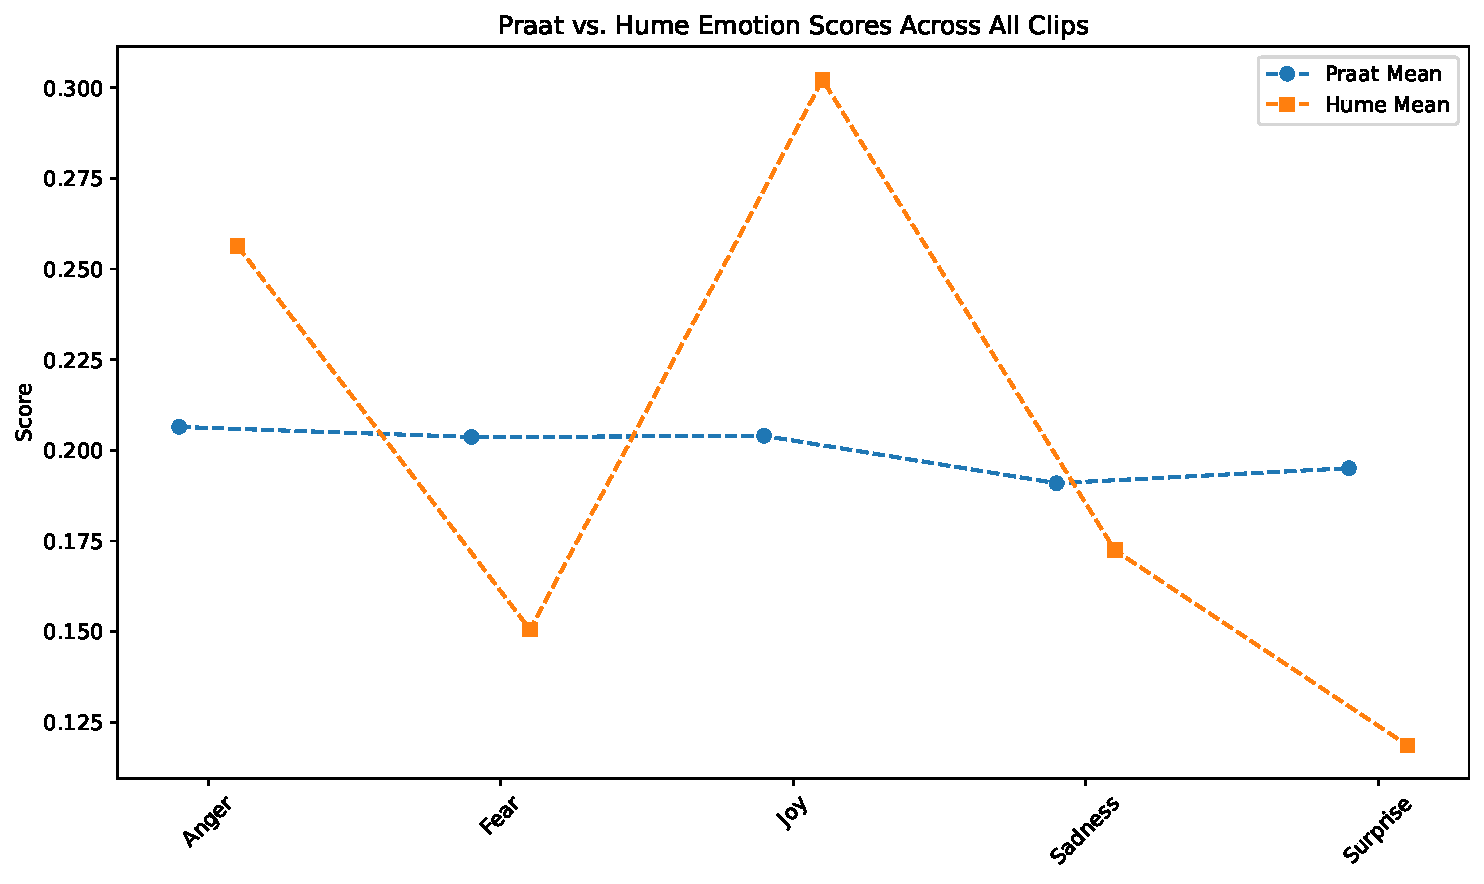
\includegraphics[width=0.7\textwidth]{png/results/rq1/praat_hume_all_clips_scatter.pdf}
    \caption{Average Score of vocal features-categorization and Hume labeling across all clips.}
    \label{fig:scatter_hume_praat}
\end{figure}

This is presented similarly in Figure Y, which presents a comparison for a single negative directed interview \texttt{id\_008\_neg}. In the same way as in Figure~\ref{fig:scatter_hume_praat}, the Praat-based scores are distributed very evenly across all emotions, while Hume assigns a higher probability to anger and lower for surprise,
with joy, sadness, and fear clustered more closely. Despite the fact that the score diversity between the Hume-labeled emotions are relatively moderate - approximately 0.10 between anger and sadness/joy, and around 0.15 between surprise and sadness/joy - the probabilities are still more diverse and provide a more interpretable output. The variability could be considered more reflective of potential emotional nuances in the interview. 

These findings demonstrate that our vocal feature-based categorization lacked sensitivity and adaptability when applied to our interview-based Swedish speech data. As a result, subsequent analyses focused on direct comparisons between raw vocal features and AI-predicted emotions, instead of relying on this flawed categorization method. 
\begin{figure}[H]
    \centering
    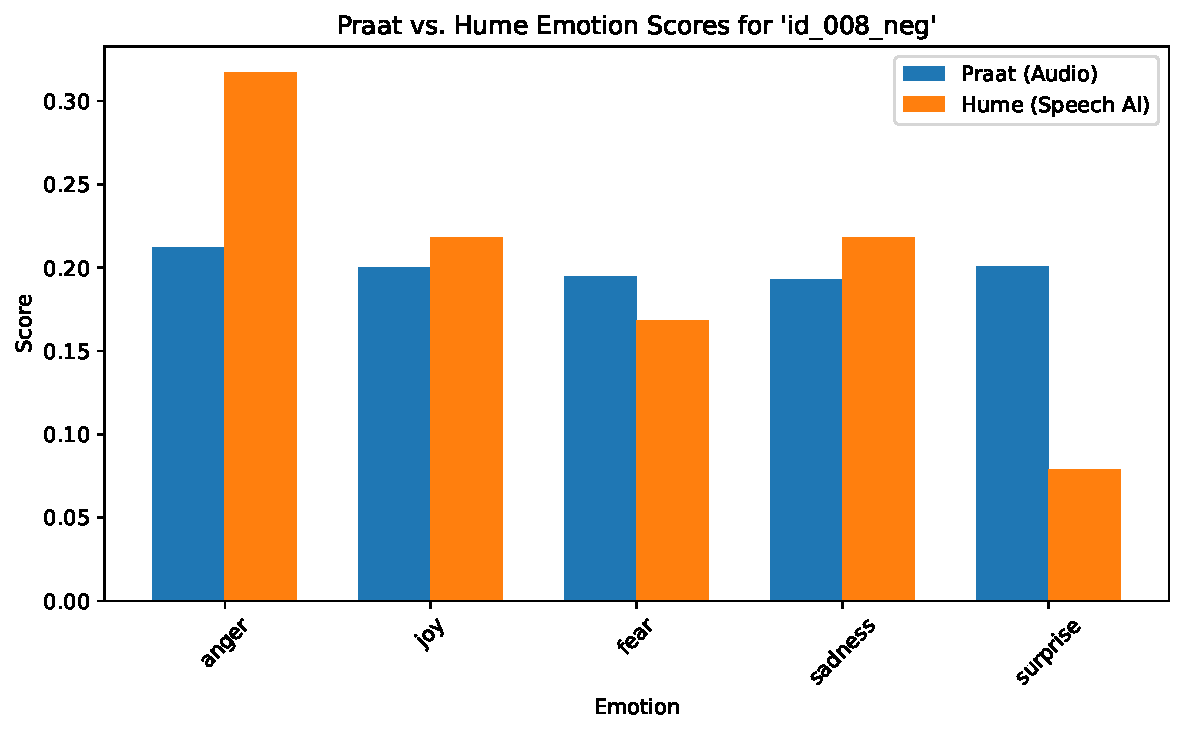
\includegraphics[width=0.7\textwidth]{png/results/rq1/id_008_neg_praat_hume_comparison.pdf}
    \caption{Vocal feature-categorization vs. Hume for single clip.}
    \label{fig:praat_hume_008}
\end{figure}

\subsection{ANOVA Summery of Vocal Features Across Emotions}
An ANOVA was implemented to further examine whether essential vocal features varied across AI-labeled emotions. This was conducted on pitch, intensity, HNR, jitter, and shimmer. The results are summarised in Table~\ref{tab:anova-rq1} and showed that none of the features showed statistically significant differences between the five Hume emotion categories (all p-values > 0.23). To confirm these findings, Tukey HSD tests were conducted and resulted in no pairwise comparisons between emotion labels with significant difference. 

\begin{table}[H]
    \centering
    \begin{tabular}{l|r|rrr}
    \multicolumn{1}{c|}{\textbf{Feature}} & \multicolumn{1}{c|}{\textbf{ANOVA p-value}} & \multicolumn{1}{c}{\textbf{Significant Differences}} &  &  \\ \cline{1-3}
   
    mean\_pitch\_hz                      & 0,4435                                     & No                                                   &  &  \\
    mean\_intensity\_db                  & 0,5793                                     & No                                                   &  &  \\
    mean\_hnr\_db                        & 0,2327                                     & No                                                   &  &  \\
    jitter\_local                        & 0,7797                                     & No                                                   &  &  \\
    shimmer\_local                       & 0,385                                      & No                                                   &  & 
    \end{tabular}
    \caption{ANOVA table for vocal features variance across emotions}
    \label{tab:anova-rq1}
\end{table}
These results imply that within our dataset of spontaneous speech during interviews, the average values of the acoustic features did not systematically vary according to AI-labeled emotions. This could indicate that emotional expression in conversations during interview circumstances is either: 
\begin{itemize}
    \item More subtle than in controlled studies.
    \item Features like pitch and intensity fluctuate instead of differing consistently at the audio clip level. 
    \item A deficient set of vocal features were extracted for these analyses. 
\end{itemize}
The lack of variance in these results does not align with findings in controlled settings \autocite{Ekberg2023}, where clear differences in vocal features were found between different emotional states. 

\subsection{Correlation Between Vocal Features and Hume AI Emotion Scores}
Considering the limitations that had been identified in our vocal feature-based emotion categorization function, subsequent analyses shifted focus towards examining direct correlation between raw acoustic features and AI-predicted emotions. Instead of applying predefined vocal emotion mappings to rely on, essential vocal markers have been investigated to obtain an understanding of how these correlate with Hume AI’s emotion scores across our dataset. 

\subsubsection{Composite Correlation Overview}
Figure~\ref{fig:composite} illustrates a composite correlation analysis, including Pearson correlation coefficients (r) between two acoustic features - pitch and intensity - and the given emotion categories that are filtered from Hume AI. Even if the correlations are generally moderate, certain patterns appear which aligns with previous findings in vocal emotion research. 
\begin{figure}[H]
    \centering 
    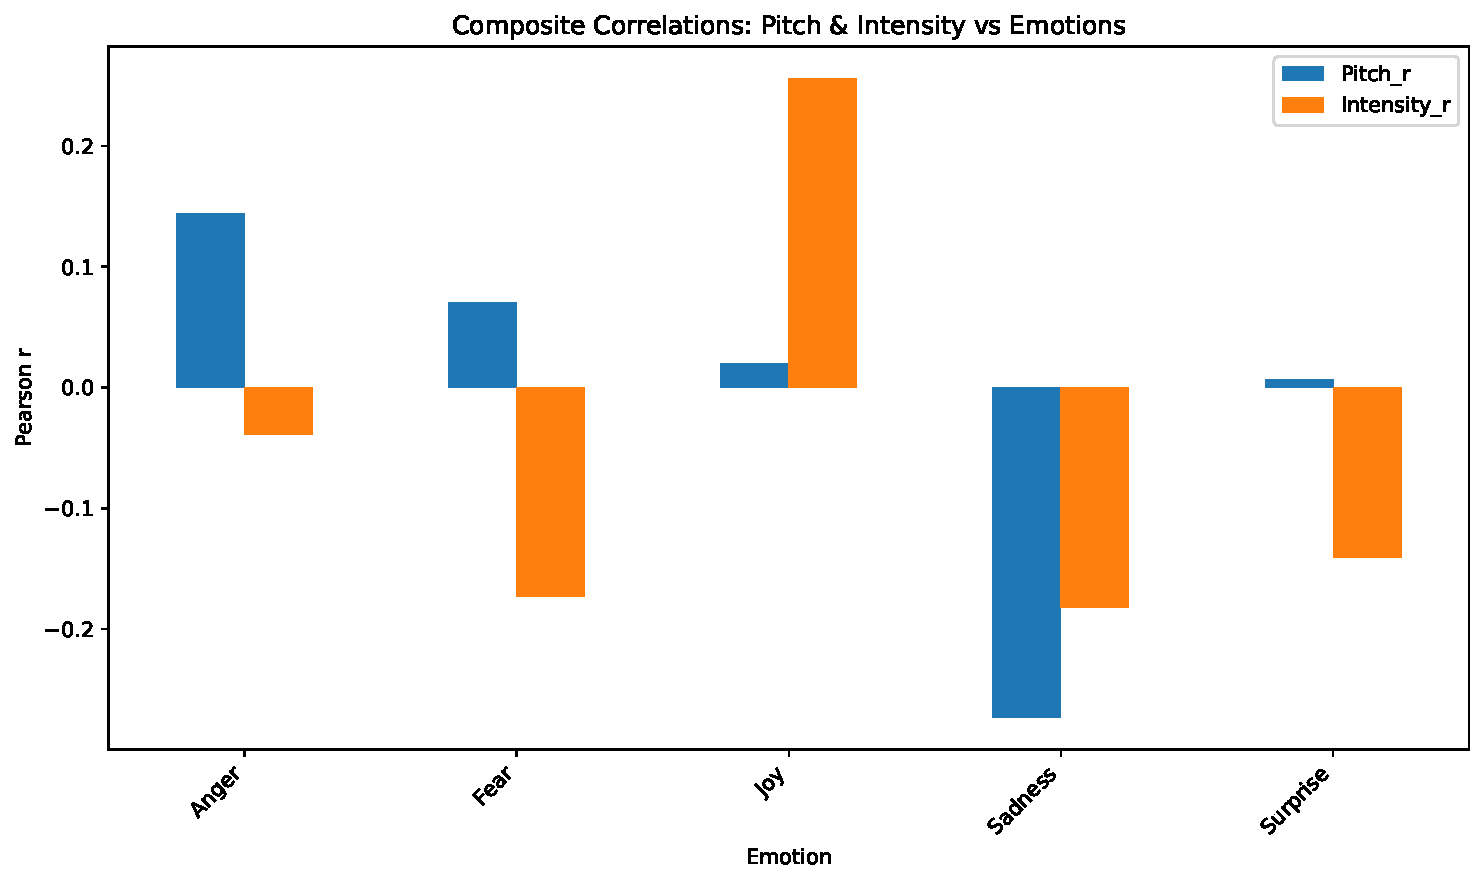
\includegraphics[width=0.6\textwidth]{png/results/rq1/composite_correlations.pdf}
    \caption{Composite correlation analysis}
    \label{fig:composite}
\end{figure}

Particularly intensity shows a positive correlation with joy, and suggests that higher vocal intensity tends to co-occur with AI detected happiness. In contrast, intensity shows a negative correlation with emotions such as sadness and fear, which is aligned with the expectations that these emotions are generally expressed with lower vocal energy. 

For pitch, a minor positive correlation is found in correlation with anger and fear, also reflecting expectations reported in prior research, where higher pitch is associated with heightened arousal states, for example anger. A negative correlation between pitch and sadness is shown, also supporting the prior findings where sadness is linked to lower pitch. 

However, the correlation strength is weak across all emotions, without values that indicate a strong linear association. This indicates, as our previous results, that single acoustic features like pitch and intensity alone are insufficient markers of emotional states when detected by speech emotion recognition systems, in the context of conversational, but interviewed, speech. 

\subsubsection{Supporting observations from individual clips}

For a more concrete illustration of the prior tendencies stated, two interview recordings were analyzed in detail. The purpose was to examine whether emotional shifts become more apparent when evaluating shorter time segments within individual speakers, compared to the weaker correlations observed at the dataset level.

In Figure~\ref{fig:pitch-4-pos} and \ref{fig:intensity-4-pos}, data is demonstrated from a positively directed interview \texttt{id\_004\_pos}, female, which shows that increases in pitch and intensity considerably often correlate with higher joy probabilities by Hume AI. While the correlation is not consistent throughout the recording, these moment-to-moment variations reflect the general expectation that higher vocal energy is associated with positive emotional expression. 

\begin{figure}[H]
    \centering
    \begin{subfigure}[b]{0.47\textwidth}
        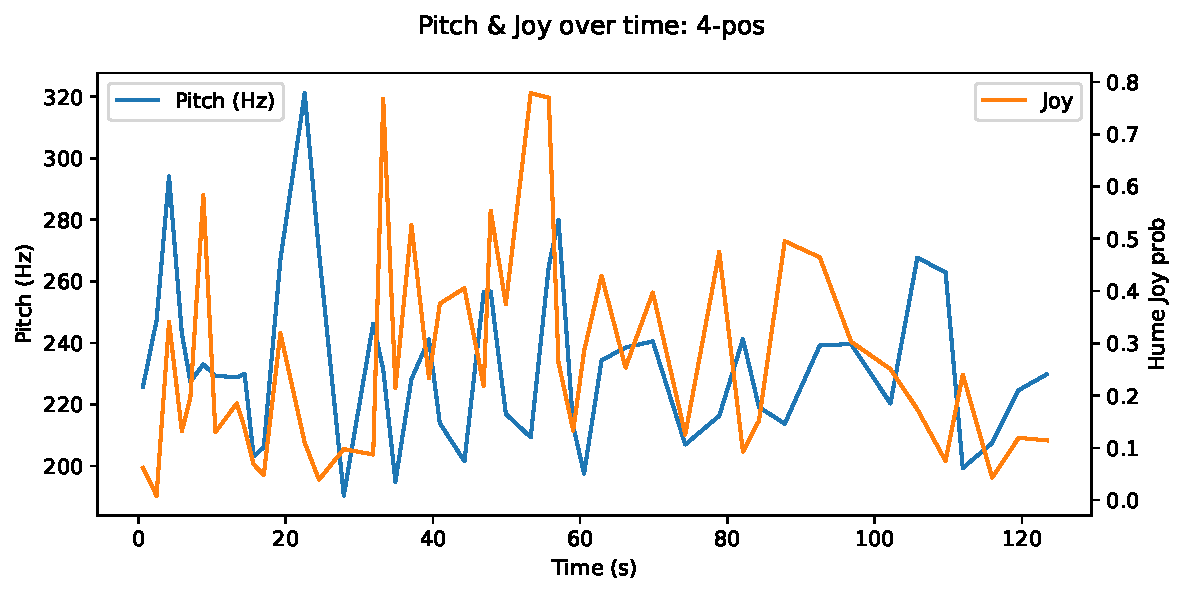
\includegraphics[width=\linewidth]{png/results/rq1/pitch_joy_4-pos.pdf}
        \caption{Pitch(Hz) and Hume label joy over time. Clip 4-pos}
        \label{fig:pitch-4-pos}
    \end{subfigure}
    \hspace{0.04\textwidth}
    \begin{subfigure}[b]{0.47\textwidth}
        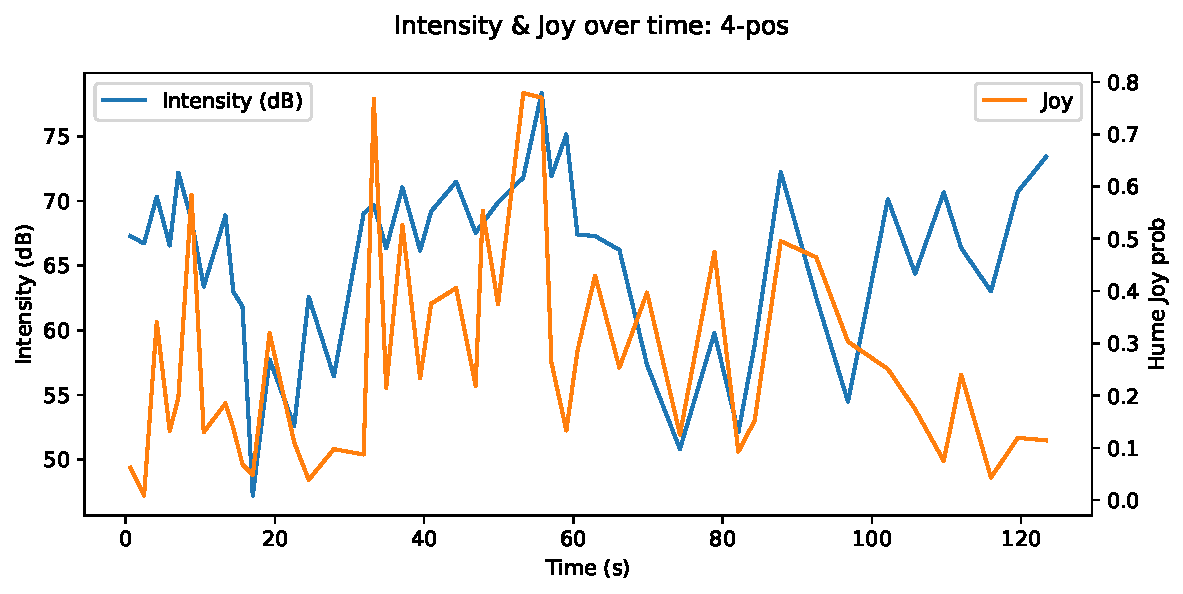
\includegraphics[width=\linewidth]{png/results/rq1/intensity_joy_4-pos.pdf}
        \caption{Intensity(dB) and Hume label joy over time. Clip 4-pos}
        \label{fig:intensity-4-pos}
    \end{subfigure}
\end{figure}

Similarly, Figure~\ref{fig:pitch-15-neg} and \ref{fig:intensity-15-neg} and \ref{fig:z-score-15} present data from a negatively directed interview \texttt{id\_015\_neg}, male. Here, clear peaks in pitch and intensity correspond with increased anger probabilities. These results are partly aligned with prior research on vocal markers of high-arousal negative emotions, such as raised pitch and loudness during expressed anger. 

\begin{figure}[H]
    \centering
    \begin{subfigure}[b]{0.47\textwidth}
        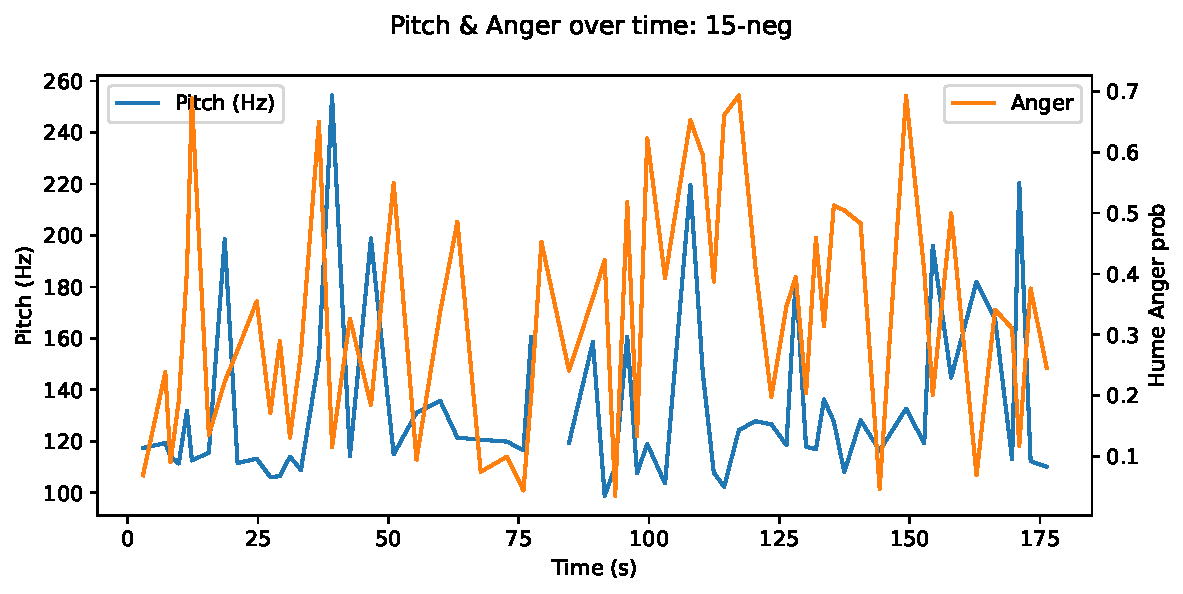
\includegraphics[width=\linewidth]{png/results/rq1/pitch_anger_15-neg.pdf}
        \caption{Pitch(Hz) and Hume label joy over time. Clip 15-neg}
        \label{fig:pitch-15-neg}
    \end{subfigure}
    \hspace{0.04\textwidth}
    \begin{subfigure}[b]{0.47\textwidth}
        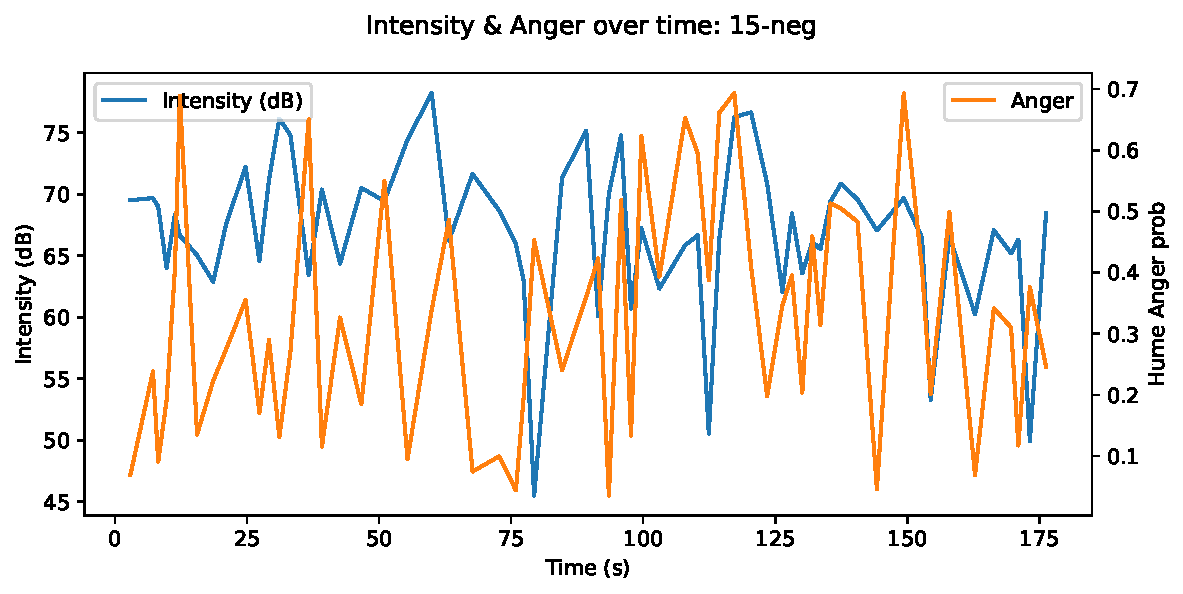
\includegraphics[width=\linewidth]{png/results/rq1/intensity_anger_15-neg.pdf}
        \caption{Intensity(dB) and Hume label joy over time. Clip 15-neg}
        \label{fig:intensity-15-neg}
    \end{subfigure}
\end{figure}

Additionally, Figure C illustrates z-score fluctuations of key vocal features for clip 13-neg. For this interview, several segments exceed +-1 standard deviation from the baseline, especially for pitch, intensity, and shimmer. These flagged moments align frequently with the emotion probabilities of Hume, which strengthens the link between vocal patterns and perceived emotional intensity. 

The z-score fluctuation diagram Figure \ref{fig:z-score-15} illustrates the segments further where vocal features significantly deviate from baseline levels, in patterns aligned with associated high-arousal negative emotions such as raised pitch and loudness. 

\begin{figure}[H]
    \centering 
    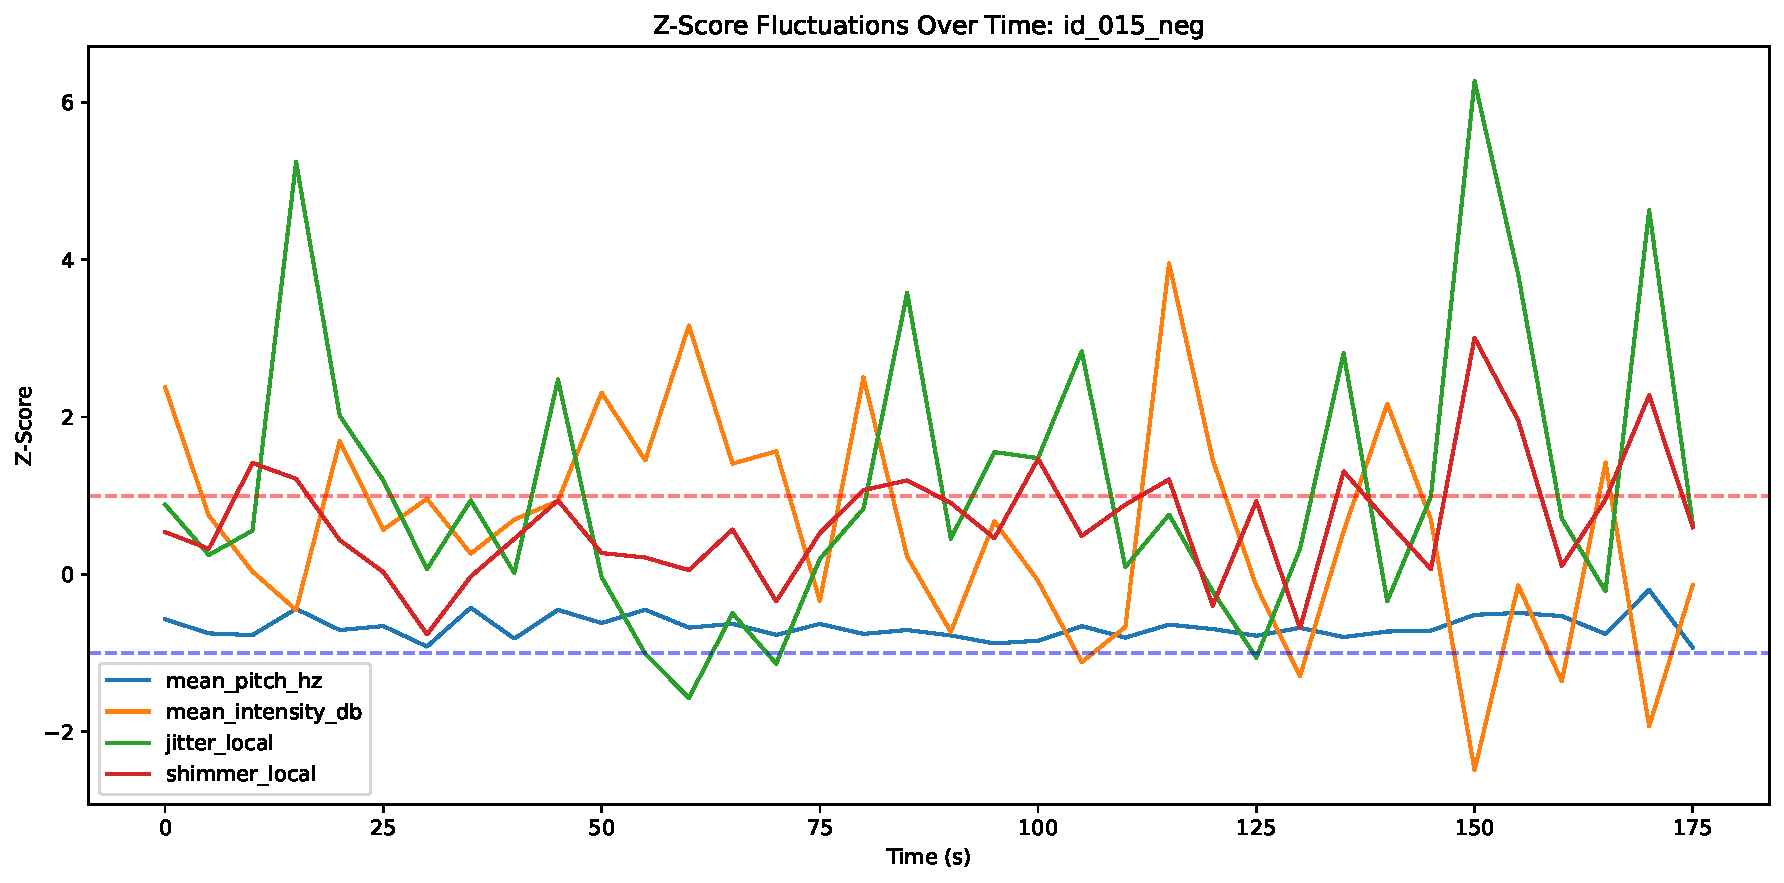
\includegraphics[width=0.7\textwidth]{png/results/rq1/zscore_fluctuations_id_015_neg.pdf}
    \caption{Z-score}
    \label{fig:z-score-15}
\end{figure}

\subsubsection{Summery}
This supports the idea that analyzing how vocal features change over time  can provide more meaningful insights into emotional expression in conversational, partly spontaneous speech during interviews compared to only using overall clip-level statistics.